\andi{Look out for words like `significantly'}

We have developed a technique, \simulator, for automatically identifying
a minimal sequence of inputs responsibly for triggering a given
bug. Here we detail the specifics
of \simulator.

We start by describing an example bug in the Floodlight
open source control platform~\cite{floodlight_bug} to illustrate the mechanics
of our technique. Floodlight is distributed across
multiple controllers for high availability, and provides support for
virtualization. Switches maintain one hot connection to a master controller and
several cold connections to replica controllers. The \emph{master} holds the
authority to modify the configuration of switches, while the other
controllers are in \emph{backup} mode and do not perform any changes to the
switch configurations unless they detect that the master has crashed.

\begin{figure}[t]
    %\hspace{-10pt}
    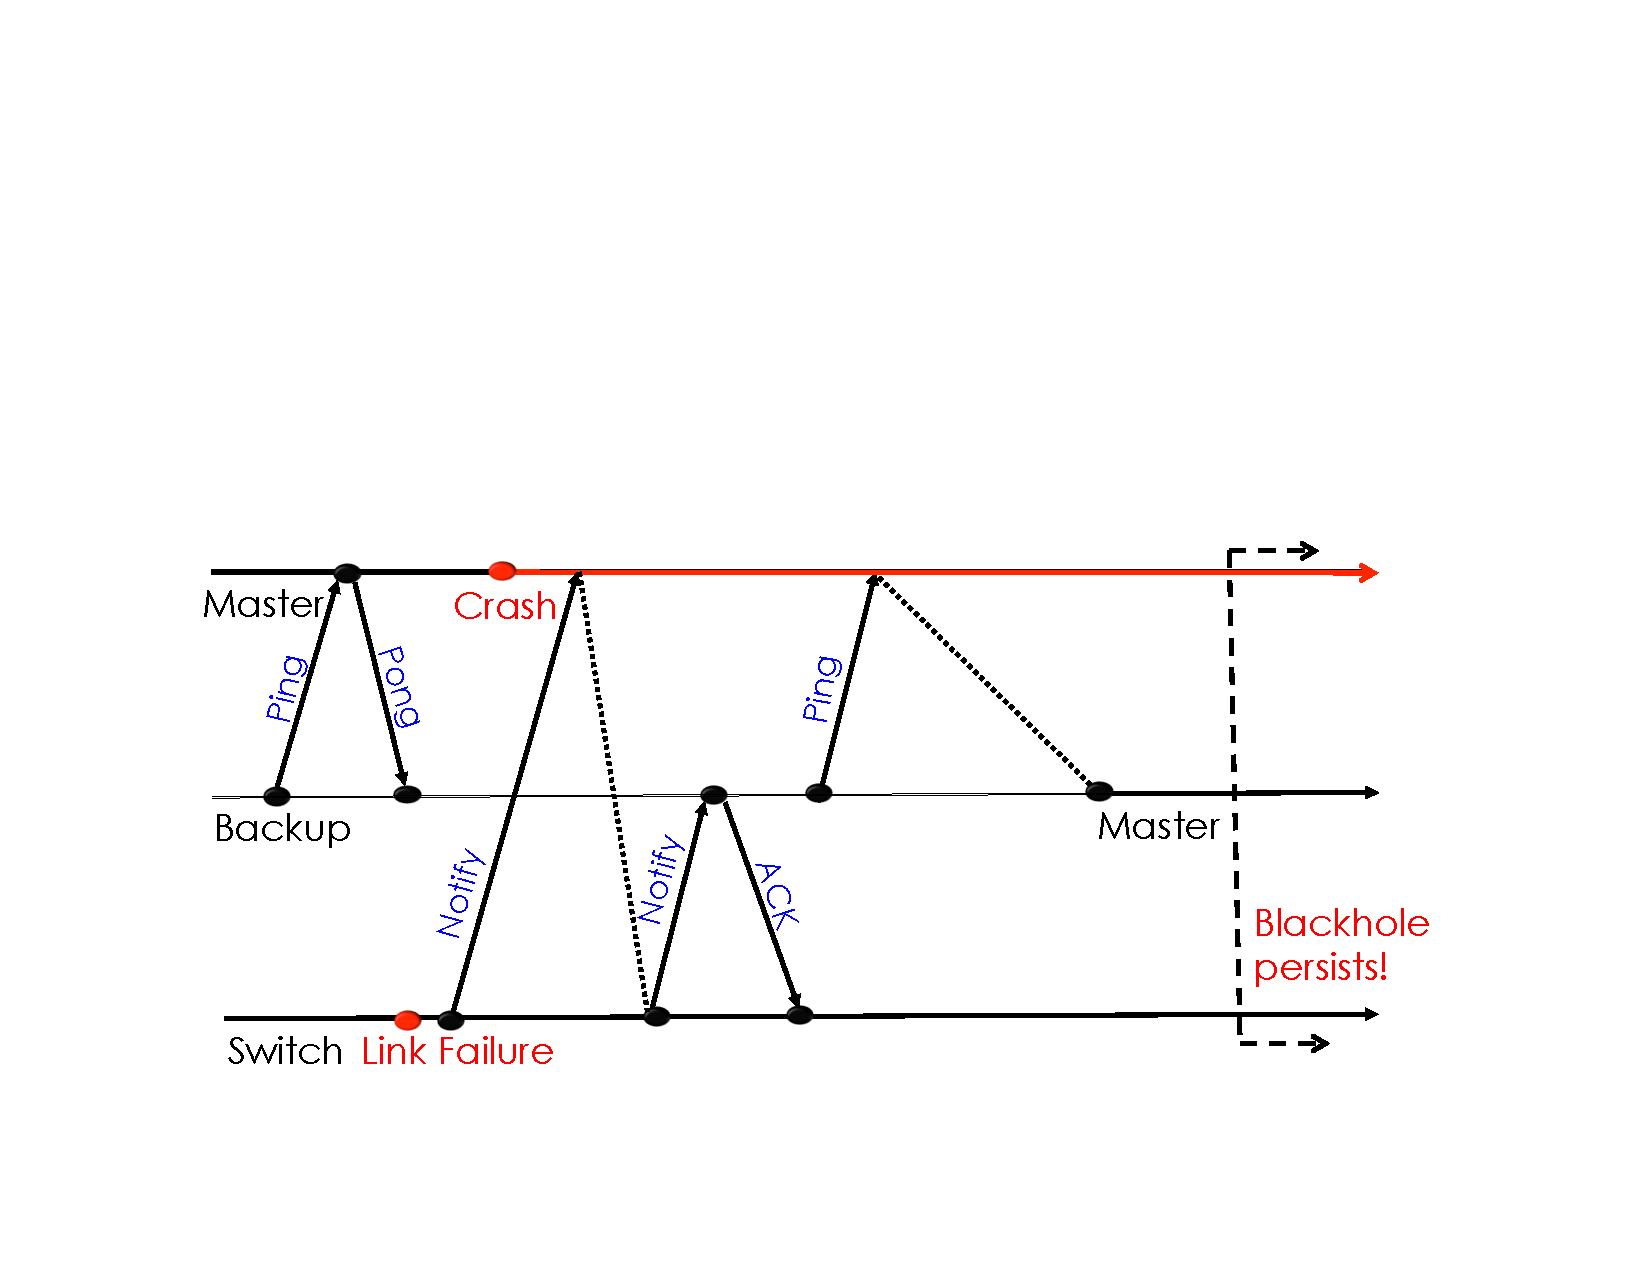
\includegraphics[width=3.25in]{../diagrams/case_study/example_bug.pdf}
    \caption[]{\label{fig:example} Floodlight failover bug. External inputs
               are depicted as red dots, internal events are depicted as black
               dots, and the dotted messages line depicts a timeout.}
\end{figure}

The failover logic in Floodlight is not implemented correctly, leading to the
following race condition\footnote{Note that this issue was
originally documented by the developers of Floodlight~\cite{floodlight_bug}} depicted in
Figure~\ref{fig:example}:
a link fails (E1), and the switch attempts to notify the controllers (E2,E4) shortly after the master
controller has died (E3), but before a new master has been selected (E6). In this case, all live controllers are in
the backup role and will not take responsibility for updating the switch
flow table (E5). At some point, a backup notices the master failure and
elevates itself to the master role (E6). The new master will proceed to manage
the switch, but without ever clearing the routing entries for
the failed link (resulting in a persistent blackhole).

There were only two external inputs (E1,E3) shown in our example.
Even relatively simple cases may contain extraneous inputs, making it difficult
for a troubleshooter to reason about the underlying root cause.
In the worst case, operators may need to examine logs from a production
network, which contain a substantial number of hardware failures, topology changes,
and other potential triggering events,
all of which may appear characteristic of normal operating
conditions at first glance; assuming 8.5 network error events per
minute~\cite{Greenberg:2009:VSF:1592568.1592576}, 500 VM migrations per
hour~\cite{Soundararajan:2010:CBS:1899928.1899941}, and a relevant execution
history of one hour, there would be over 1000 inputs to the system
reflected in the log.

Given a trace of the system execution similar to the Floodlight case,
our goal is to prune events that are not
necessary for triggering errant behavior. We define errant behavior in terms
of {\em correctness violations}:
configurations of the network that are inconsistent
with the policy. In the example, the correctness violation is between a
reachability policy specified in the logical view (``A can talk to B'')
and the blackhole in the physical network (``A's packets to B enter the
blackhole and do not arrive at B'').

We have developed a technique to automatically perform this pruning.
Specifically, our technique identifies a minimal sequence of inputs
to the controllers that is sufficient for triggering a known correctness violation. We
refer to such inputs as a {\em minimal causal sequence} (MCS). Going back to our example,
suppose the log includes many more (extraneous) inputs. Whenever an
extraneous event is pruned, the blackhole will still persist. When
the controller crash is pruned, the blackhole will be resolved properly, and
when the link failure is pruned, no blackhole will occur. The MCS returned
is therefore the controller crash and the link failure in conjunction.

\subsection{Delta Debugging}
\label{subsec:algorithm}

Delta debugging~\cite{Zeller:1999:YMP:318773.318946}, a technique from the
software engineering community, gets us part of the way
there: given a single input (\eg~an HTML page)
for a non-distributed program (\eg~Firefox), it performs a divide-and-conquer
search, repeatedly running the program on subsets of the input
until it finds a minimal subset (\eg~a single tag) that is sufficient
for triggering a known bug. Specifically, it finds a 1-minimal
(locally minimal) causal sequence~\cite{Zeller:1999:YMP:318773.318946},
meaning that if any input from the sequence is pruned, no correctness violation
occurs. The delta debugging algorithm is shown in
Figure~\ref{fig:ddmin} (with `$test$' replaced by `$replay$').

\begin{figure*}[t]
\caption{Automated Delta Debugging Algorithm From~\cite{Zeller:1999:YMP:318773.318946}}
\begin{boxedminipage}{\textwidth}
Input: $\cfail$ s.t. $\cfail$ is a trace and $\test(\cfail) = \FAIL$. Output: $\dfail
= \ddmin(\cfail)$ s.t. $\dfail \subseteq
\cfail$, $\test(\dfail) = \FAIL$, and~$\dfail$ is 1-minimal.
\begin{align*}
\ddmin(\cfail) &= \ddmin_2(\cfail, \emptyset) \quad \text{where} \\
\ddmin_2(\dfail, R) &=
\begin{cases}
\dfail & \text{\hphantom{else }if $|\dfail| = 1$ (``base case'')} \\
\ddmin_2\bigl(\done, R\bigr) &
\text{else if $\test(\done \cup R) = \FAIL$ (``in $\done$'')} \\
\ddmin_2\bigl(\dtwo, R\bigr) &
\text{else if $\test(\dtwo \cup R) = \FAIL$ (``in $\dtwo$'')} \\
\ddmin_2\bigl(\done, \dtwo \cup R\bigr) \cup \ddmin_2\bigl(\dtwo, \done \cup
R\bigr) & \text{otherwise (``interference'')}
\end{cases}
\end{align*}
\begin{center}
where $\test(T)$ denotes the state of the system after executing the trace $T$,
$\FAIL$ denotes a correctness violation, \\
$\done \subset \dfail$, $\dtwo \subset \dfail$, $\done \cup \dtwo = \dfail$, $\done \cap
\dtwo = \emptyset$, and $|\done| \approx |\dtwo| \approx |\dfail| / 2$
hold.
\end{center}
\end{boxedminipage}
\label{fig:ddmin}
\end{figure*}

\eat{ % Original O(n^2) algorithm
\begin{figure*}[t]
\caption{Minimizing Delta Debugging Algorithm From~\cite{Zeller:2002:SIF:506201.506206}}
\begin{boxedminipage}{\textwidth}
Input: $\cfail$ s.t. $\cfail$ is a trace and $\test(\cfail) = \FAIL$. Output: $\dfail
= \ddmin(\cfail)$ s.t. $\dfail \subseteq
\cfail$, $\test(\dfail) = \FAIL$, and~$\dfail$ is 1-minimal.
\begin{align*}
\ddmin(\cfail) &= \ddmin_2(\cfail, 2) \quad \text{where} \\
\ddmin_2(\dfail, n) &= 
\begin{cases}
\ddmin_2(\Delta_i, 2) & \text{\hphantom{else }if $\exists i \in \{1, \dots, n\} \cdot \test(\Delta_i) = \FAIL$ (``reduce to subset'')} \\
\ddmin_2\bigl(\nabla_i, \max(n - 1, 2)\bigr) & 
\text{else if $\exists i \in \{1, \dots, n\} \cdot \test(\nabla_i) = \FAIL$ (``reduce to complement'')} \\
\ddmin_2\bigl(\dfail, \min(|\dfail|, 2n)\bigr) & \text{else if $n < |\dfail|$ (``increase granularity'')} \\
\dfail & \text{otherwise (``done'').}
\end{cases}
\end{align*}
where $\test(T)$ denotes the state of the system after executing the trace $T$,
$\FAIL$ denotes a correctness violation, \\
$\nabla_i = \dfail - \Delta_i$, $\dfail = \Delta_1 \cup \Delta_2 \cup \dots \cup \Delta_n$, all
$\Delta_i$ are pairwise disjoint sequences of inputs, and $\forall \Delta_i \cdot |\Delta_i| \approx |\dfail| / n$
holds.
\end{boxedminipage}
\label{fig:ddmin}
\end{figure*}
}

Our problem differs from the original formulation of delta debugging in two dimensions.
First, input to SDN controllers is spread
across time: it includes many messages, and depends on subtle causal
relationships. Second, the input is spread across space: it involves
many concurrently running nodes.
In the rest of this section, we describe how we
replay inputs to control software,
cope with alterations to the causal history of an execution, and check
for correctness violations. In \S\ref{sec:architecture}, we describe concrete
ways \simulator~can be put to use.

\subsection{Simulation}
\label{subsec:simulation}

Unlike the example applications described
by Zeller et al.~\cite{Zeller:2002:SIF:506201.506206}, the system we are troubleshooting is not a
single program--it is all the nodes and links of a distributed system,
including controllers, switches, and end-hosts. Replaying traces
on an actual network would be prohibitively costly and overly prone to
non-deterministic behavior. We therefore simulate the entire control-plane,
with support for minimal data-plane behavior,
in a single process. We then run the control software on
top of this simulator and connect the software switches to the controllers as if they were true
network devices, such that the controllers believe they are configuring a true
network. This setup allows the simulator to interpose on all communication
channels, enabling fine-grained control over message orderings. The overall
simulation architecture is depicted in
Figure~\ref{fig:architecture}.

\begin{figure}[t]
    %\hspace{-10pt}
    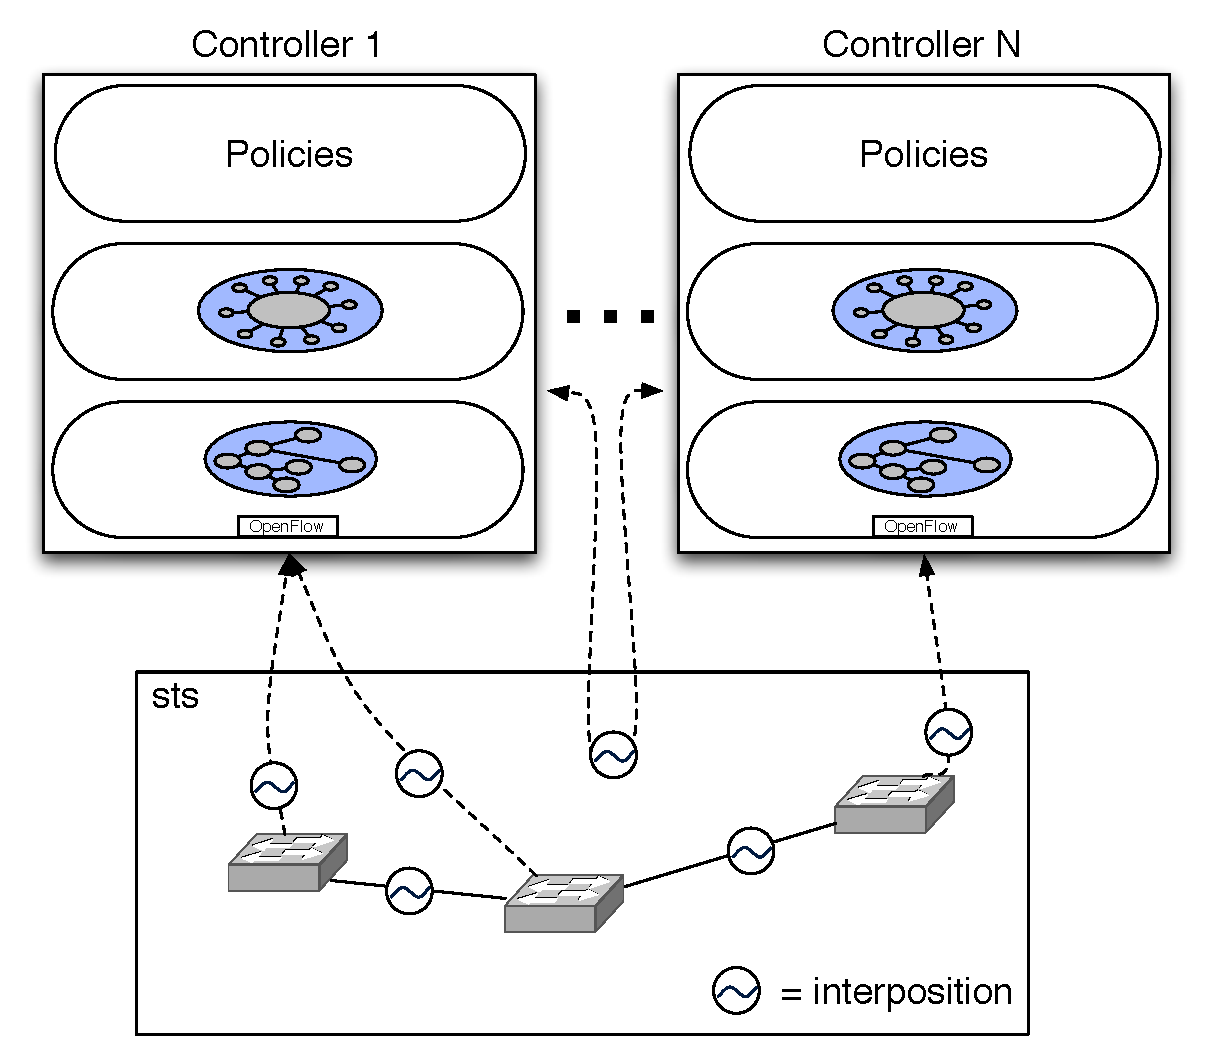
\includegraphics[width=3.25in]{../diagrams/architecture/Debugger_Architecture.pdf}
    \caption[]{\label{fig:architecture} Simulation infrastructure. Dataplane
    devices run in software, and all communication channels are
    interposed upon.}
\end{figure}

Given a sequence of inputs (\eg~link failures, controller crashes, host migrations,
or policy changes) and an invariant checking probe (provided by frameworks
such as HSA~\cite{hsa,hsa_realtime} or Anteater~\cite{anteater,khurshid2012veriflow}), the simulator invokes
the delta debugging algorithm to identify the minimal causal set. The
simulator is then responsible for replaying intermediate input subsequences
chosen by delta debugging. For example, link failures are
reproduced by disconnecting the edge in the simulated network, and sending a
port status message from the adjacent switches to their parent controller(s).

\subsection{Replay}
\label{subsec:replay}

The timing of the inputs injected by the simulator is crucial for ensuring that the
execution is the same as the original run. Na\"ively injecting inputs often fails to
trigger the original correctness violation, even without having pruned any
events. In particular, we tried and failed to reproduce errors when scheduling inputs
with the following simple algorithm:
\begin{align*}
t'_0 = 0 \\
t'_i = t'_{i-1} + |t_{i} - t_{i-1}|
\end{align*}
where $t'_i$ is the simulation's clock value when it injects the $i^{th}$ input, and $t_i$ is
the timestamp of the $i^{th}$ input from the original run. In other words, simply
maintaining the relative timing between inputs is not sufficient.

The problem with the simple scheduling algorithm is that it does not take into
account events that are internal to the control software, such as
message receipts, timers going off, or internal state
changes like the backup node in the Floodlight example deciding to elevate itself to master.
Consider for example that if a controller's garbage collector happens to run
while we replay inputs, it is feasible that the delicate ordering between
inputs internal events would be perturbed, resulting in a different output.

Formally, we need to inject an external input $e$ at exactly the point when all other
events (both external and internal) that precede it in the happens-before
relation ($\{i \mid i \rightarrow e\}$) from the original execution have occurred.
While the input and internal events from the original run are given to us,
we become aware of internal events throughout replay by
(i) monitoring
control message receipts between controllers and between switches and
controllers, and (ii) interposing on the controllers' logging library and notifying the
simulation process whenever log statement (which serve to mark relevant state
transitions) is executed. Note that to achieve truly deterministic
replay, these log statements would need to
be highly granular, capturing information such as thread scheduling decisions;
we show in \S\ref{subsec:case_studies}
however that pre-existing, course granular log statements are sufficient to
successfully reproduce many bugs.\footnote{We discuss this problem further in \S\ref{subsec:domain_knowledge}}
%Note that the developer must provide enough logging statements
%so that relevant internal state changes are captured and visible to our
%tool.

\subsection{Fingerprinting}
\label{subsec:fingerprinting}

Event scheduling is made substantially more complicated by the fact
that the delta debugging algorithm is pruning inputs from the history of the
execution, thereby changing the resulting internal events generated by the control
software. One implication of this is that the syntax of the internal events may differ
slightly from their equivalent internal events in the original
execution. Consider for example that sequence numbers of control packets may
all differ by one if a single control message in the beginning of the trace
does not occur.

Our solution is to define domain-specific masks over
semantically extraneous\footnote{Extraneous with respect to comparing two
separate traces. For example, the buffer id is chosen at random, so
it is meaningless to compare buffer ids across separate runs. One consequence
of masks is that bugs involving masked fields are outside the purview of
\simulator.} fields of
the message. A few examples of masked fields are shown
in Table~\ref{tab:fingerprints}. These masks define equivalence classes
of internal events, which allow us to compare different runs of the simulation.
Formally, we consider an internal event $i'$ observed in an altered trace
equivalent to an internal event $i$ from the original trace iff all unmasked
fields have the same value
and $i$ occurs between $i'$'s preceding and succeeding inputs in the
happens-before relation.

\begin{figure}[t]
    %\hspace{-10pt}
    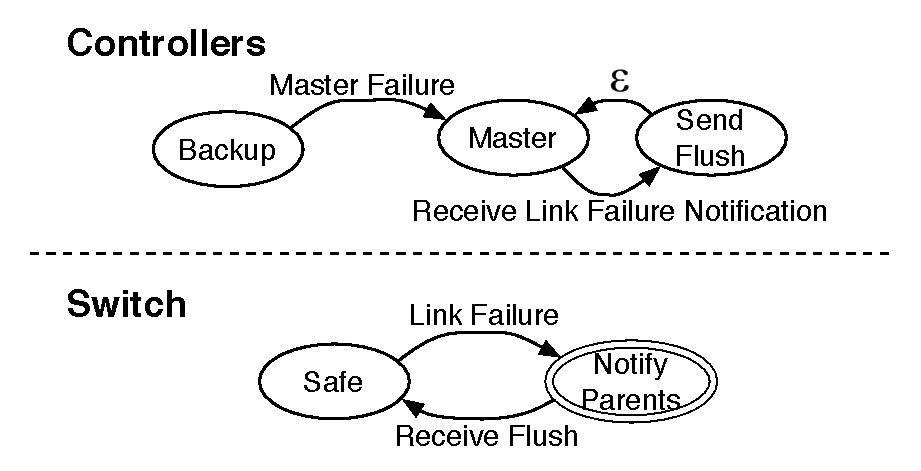
\includegraphics[width=3.25in]{../diagrams/state_machines/controller_switch.pdf}
    \caption[]{\label{fig:state_machines} Simplified state machines for the switch and
    controllers in the example Floodlight bug. Double outlined states
    represent presence of the blackhole.}
\end{figure}

\begin{table}
\centering
\begin{tabular}{|l|l|}
\hline
Internal message & Masked values \\
\hline
OpenFlow headers & transaction id\\
OpenFlow FLOW\_MODs & cookie, buffer id \\
Log statements & varargs parameters to printf \\
\hline
\end{tabular}
\caption{Example internal messages and their masked values. The masks serve to
define equivalence classes.}
\label{tab:fingerprints}
\end{table}

\subsection{Coping With Divergence}
\label{subsec:divergence}

A deeper implication of altering the original trace is that
some internal events from the original run may not occur after
pruning certain inputs--conversely, new internal events not present in the original run
may occur. Consider the simplified state machines for the switch and
controllers from the Floodlight case shown in
Figure~\ref{fig:state_machines}. If link failure input is pruned, the
switch will not make the transition to `Notify Parents', and the master will
consequently not make the transition to and from `Send Flush'. Without being
able to equate events from alternate histories, it is nearly impossible to resolve
divergences like this in a way that ensures that the original bug is still
triggered.

We have developed two event scheduling algorithms to account for altered
internal events. The first is simpler, but somewhat less robust. We refer to it as
\emph{waiting replay}, and it is shown in Figure~\ref{fig:simple_algorithm}.
Simply put, it waits for internal events matching those in the original run,
but times out and proceeds if they do not occur.

\begin{figure}
\begin{boxedminipage}{\linewidth}
\begin{Verbatim}[commandchars=\\\{\}]
for e\textsubscript{i} in trace:
  if e\textsubscript{i} is an internal event:
    \textDelta = |e\textsubscript{i}.time - e\textsubscript{i-1}.time| + \textepsilon
    wait up to \textDelta seconds for e\textsubscript{i}
  else: // input
    inject e\textsubscript{i}
\end{Verbatim}
\end{boxedminipage}
\caption{Waiting Replay Algorithm}
\label{fig:simple_algorithm}
\end{figure}

In most cases waiting replay successfully reproduces the original correctness
violation, assuming \textepsilon~is larger than variations in execution speeds
between internal events. If the value of \textepsilon~is too large, however, we may end up
waiting too long for the happens-before predecessors of an input $e_i$ such that a
successor of $e_i$ occurs before we have injected $e_i$,
potentially resulting in an altered output.
% \sam{Is it worth noting that this isn't necessarily a problem? If a successor occurs, it means it wasn't causally related to $e_i$, but the ordering still might matter for further successors.}

Our second event scheduling algorithm addresses this possibility, but
adds a factor of $n$ in the number of replayed inputs to the overall
runtime. We refer to it as \emph{peeking replay}, and it is shown in Figure~\ref{fig:peek}.
Simply put, peeking replay
attempts to precompute which internal events are and aren't going to occur
between any adjacent pair of inputs
so that it can know exactly how long to wait before injecting inputs in the
final replay.

\begin{figure}
\begin{boxedminipage}{\linewidth}
\begin{Verbatim}[commandchars=\\\{\}]
inputs = [e\textsubscript{1}, e\textsubscript{2}, ..., e\textsubscript{n}]
new\_trace = []

for i in 1 to n-1:
  waiting\_replay(new\_trace + [e\textsubscript{i}], \textepsilon=0)
  start recording internal events
  \textDelta = |e\textsubscript{i+1}.time - e\textsubscript{i}.time| + \textepsilon
  wait \textDelta seconds
  remove successors of e\textsubscript{i} from \textbackslash
    recorded internal events
  new\_trace += [e\textsubscript{i}]
  new\_trace += recorded internal events

waiting\_replay(new\_trace + [e\textsubscript{n}], \textepsilon=0)
\end{Verbatim}
\end{boxedminipage}
\caption{Peeking Replay Algorithm}
\label{fig:peek}
\end{figure}

% TODO: not quite true!
In practice we employ a hybrid algorithm
that defaults to waiting replay and only
peeks during intervals where it has waited too long.
This is possible because waiting replay can always detect when it has
waited too long upon observing a successor of the input to be injected.
Although the hybrid algorithm has the same worst case runtime as peeking
replay, the average case runtime is significantly better.

Waiting and peeking replay both need to account for the pathological case
where {\em multiple} internal events in the same
equivalence class a single internal event in the original execution.
Ambiguous equivalences mean that more than one possibility exists for where
the next input should be
injected while still maintaining happens-before constraints. For example, if $i_2$ and $i_3$ are internal events observed
during replay that are both in the same equivalence class as a single event $i_1$ from the
original run, one might inject the next input after $i_2$ or after $i_3$.
As we have proven elsewhere,\footnote{URL omitted for anonymity reasons}
all possibilities need to be explored to guarantee that if a path through the
distributed state machine leading to
the correctness violation from the original execution exists, that path will be taken. In the worst case,
this implies an exponential number of possibilities to be explored during
replay.

Luckily, ambiguous equivalent internal events are extremely rare in the
control software we evaluated, as we
show in \S\ref{subsec:runtime}. We have proven elsewhere that ambiguity only
occurs when a sub-path exists in the distributed state machine that contains two or
more equivalent internal edges without an intermediate input event edge.
We conjecture that such transitions are not common in control plane systems,
which are designed to quiesce quickly (\ie~take a small number of internal
transitions after any input event). Consider the state machines in Figure~\ref{fig:state_machines}:
it is not possible to traverse the same internal event edge (``Receive Link
Failure Notification'' or ``Receive Flush'') without traversing an
intermediate input event edge (``Link Failure'' or ``Master Failure'').
\colin{TODO: need a figure that shows generalized event scheduling}

\subsection{Complexity}
\label{subsec:complexity}

Assuming no ambiguities occur, the delta debugging algorithm terminates after
$O(log\,n)$
invocations of $replay$ in the best case, where $n$ is the number of inputs in the original
trace~\cite{Zeller:2002:SIF:506201.506206}. Each invocation of waiting replay
replays $n$ inputs, for an overall runtime of $O(nlog\,n)$ for
waiting replay. The worst case runtime of delta debugging is $O(n)$ in the
number of invocations of $replay$.
\footnote{Note that this version of delta debugging
assumes that no unresolved test
outcomes occur. We ensure that this assumption holds by filtering inputs
sequences that we know are invalid (\eg~link recoveries without a preceding
link failure), as in Section 6~\cite{Zeller:1999:YMP:318773.318946}. The
author's follow-on
paper~\cite{Zeller:2002:SIF:506201.506206} removes the need for the assumption,
but adds a factor of $N$ to the runtime.}
Therefore the overall worst case runtime is $O(n^2)$ if waiting replay is used.

Peeking replay adds another factor of $n$ to the overall runtime: for each input event
$e_i$, it invokes waiting replay with inputs $e_1,\dots,e_i$, for a total of
$n \times \frac{n+1}{2} \in O(n^2)$ replayed inputs. Therefore in the
best case, the overall runtime of delta debugging with peeking replay is
$O(nlog\,n)$, and the worst case is $O(n^3)$. Note that this extra factor of
$n$ in computational complexity can be converted to a factor of $n$ in storage
complexity if peek stores snapshots of
the controllers' state rather than replaying each prefix from the beginning.

\subsection{Parameters}
\label{subsec:params}

Both waiting and peeking replay leave an open question as to what value
\textepsilon~should be set to. In our current implementation,
we set \textepsilon~\num{somewhat arbitrarily} to $100$ milliseconds, and this has worked for \num{most} of our
failure cases. In general, larger values of \textepsilon~are preferable to
smaller values (disregarding runtime considerations), since we can always
detect when we have waited too long (\viz~when a successor of the next input
has occurred), but we cannot detect when we have timed out
early on an internal event that is in fact going to occur.

In practice we also make optimization to the overall delta debugging
algorithm: since some of the input subsequences
chosen by unmodified delta debugging may not be valid, we apply domain knowledge
about input validity to avoid exploring certain subsequences. For example, it does
not make sense to replay a link recovery event if we pruned
the link failure event that preceded it. Likewise, pruning a host migration
implies that we need to update the subsequent host migration event's source location.
Beyond component failures and host migration, other dependencies between
inputs are significantly more complicated to model.
%At the
%moment, our tool does not support policy changes or dataplane packet drops for
%this reason.

\colin{Mention that causal
annotations and selective pruning help.} \colin{Make sure we emphasize that there is no `right answer', since we're
dealing with modified histories.}

\subsection{Correspondence Checking}
\label{subsec:cc}

\num{Cut if no space.}
Finally, we need a mechanism for deciding
whether a correctness violation is present at the end of the system execution.
We refer to such an algorithm as a {\em decider}.

\Simulator~supports generic deciders (\eg~all-pairs reachability or loop detection),
provided by frameworks such as Hassel~\cite{hsa,hsa_realtime} or
Anteater~\cite{anteater,khurshid2012veriflow}.
With a small modification to the control software however, we can
extract the network policies already reflected in the
controller's data structures and thereby check a much more fine-grained set of invariants.
We refer to this technique as correspondence checking. Correspondence checking
builds on the virtual packet algebra
pioneered in headerspace analysis~\cite{hsa}.

Formally, the state of the physical network, the physical view (the
data structure maintained by the controllers for tracking the current state of the physical
network), and the
logical view (the data structure maintained by the controllers for storing
network policies in a routing table-like format) can be represented as graphs,
$G = (V, E)$. Packets are series of bits, $h \in \{0,1\}^L$ in the universe
of all possible bit sequences $H = \{0,1\}^L$,
where $L$ is the maximum number of bits in the header.

Upon receiving a packet,
forwarding elements apply a transformation function, potentially modifying
packets before forwarding them on\footnote{Multicast forwarding can expressed
by extending the range to sets of output tuples}:
\begin{align*}
T: (H \times E) \rightarrow (H \times E_{\emptyset})
\end{align*}
Here, $E_{\emptyset} \equiv E \cup \emptyset$, signifying that forwarding elements
may drop packets.

We use $\Psi$ to denote the collection of all transfer functions present in
the network at a particular point in time. In this model, network traversal is
simply repeated application of $\Psi$.
For example, if a header $h$ enters the network through edge
$e$, its state after $k$ hops will be:
\begin{align*}
\Psi^k(h,e) = \Psi(\Psi(\dots \Psi(h,e)\dots))
\end{align*}

The externally visible behavior of the network can be expressed as the
transitive closure of $\Psi$:
\begin{align*}
\Omega: (H \times E_{access}) \rightarrow (H \times E_{\emptyset}) \\
\Omega(h,e) = \Psi^{\infty}(h,e)
\end{align*}
Here, $E_{access}$ denotes access links adjacent to end-hosts.

The domain of $\Omega^{physical}$ is the set of pairs of end-hosts in the
physical network along with packets they could possibly produce (before
the packets have been encapsulated). We define $\Omega^{view}$ in exactly the same way, where
the logical hosts are abstract representations of the hosts in the physical
network. This definition depends on the observation that end-hosts are represented
in all layers, even if there is not a one-to-one mapping between the
internal vertices of $G^{virtual}$ and $G^{physical}$.

The range of $\Omega$ is the hypothetical final state of the
input packet if it were injected in the network.
We use the special value $LOOP$ to distinguish
a packet dropped by a network device from a packet entering an
infinite loop (both of which never leave the network).

In SDN, it should always be the case that:
\begin{align*}
\Omega^{view} \sim \Omega^{physical}
\end{align*}
The equivalence $\sim$ means that the final outcome of any input packet
injected at a host $a_{physical}$ in the physical network has the same hypothetical final outcome as
the same input injected at the corresponding $a_{logical}$, and vice versa.

Correspondence checking takes as input a
snapshot of both the physical network and the
controllers' state. We first modify the control software to present an
interface through which the physical and virtual views can be
extracted. The snapshot is
then obtained by pausing execution and invoking this interface.
The routing tables of forwarding elements in the views and the physical
network can then be translated into transformation functions.
Finally, we feed a symbolic packet $x^L$ to each access link of the
network.\footnote{The rules for process wildcard bits $x^n$ are defined in
the HSA paper~\cite{hsa}} The end result is a propagation graph representing
all possible paths taken by any packet injected
at the access link.

We compute $\Omega$ by traversing the resulting propagation graph. If a packet
enters a loop before exiting the network, we mark the value as
$LOOP$. Otherwise,
the leaves of the propagation graph define the final outcomes of the input
packets injected at that access link. Because network policies are defined by
configuring the logical view, any mismatch between $\Omega^{view}$ and $\Omega^{physical}$
represents an instance of a correctness violation. Note that mismatches are
unambiguous; that is, two slightly different correctness violation from
different runs of the system are always distinguishable.

Note the price of correspondence checking's generality is that it represents
a somewhat weak notion of
correctness. Correspondence checking only captures external behavior and
loops; it does not capture internal behavior such as load-balancing
over links. It also assumes that the policies as expressed by the
configuration of the logical view are correct. Finally, correspondence
checking can not verify
time-dependent policies such as ``No link should be congested more than 1\% of
the time''.

\subsection{Limitations}
\label{subsec:non_goals}

Having detailed the specifics of \simulator, we now
clarify the scope of its technique's use.

\noindent{\bf Troubleshooting vs Debugging.} Our technique is a troubleshooting tool, not a debugger;
by this we mean that \simulator{} helps identify and localize inputs that
trigger erroneous behavior, but it does not directly identify which
line(s) of code cause the error.

\noindent{\bf Bugs Outside the Control Software.} Our goal is not to find the root
cause of individual component failures in the system (\eg~misbehaving routers,
link failures). Instead, we focus on
how the distributed system as a whole reacts to the occurrence of inputs such
as component failures.
If there is a bug in your switch, you need to contact your hardware vendor;
if you have a bug in your policy specification, you need to take a closer look at what you specified.
That said, our tool can show whether switches behave the same as our software
implementation: if our tool was unable to reproduce the error, that means that
the problem was above or below the control software.

\noindent{\bf Non-determinism Within Individual Controllers.} Our tool is not designed to reproduce bugs
involving non-determinism within a single controller (\eg~race-conditions between threads);
we focus on coarser granularity errors (\eg~incorrect failover logic), which we find plenty of
in \S\ref{subsec:case_studies}. The upshot of
this is that our technique is not able to minimize all possible failures, such as
data races between threads.
Nonetheless, the worst case for us is that the developer ends up with what they started:
an unpruned log. That said, if the developer is willing to instrument their system to
provide finer granularity log messages (\cf~\cite{Geels:2006:RDD:1267359.1267386}),
our approach readily supports deterministic replay.

\noindent{\bf Globally vs Locally Minimal Input Sequences.}
Our approach is not guaranteed to find the globally minimal
causal sequence from an input trace, since this requires $O(2^N)$ computation in the worst case.
The delta debugging algorithm we employ however is guaranteed to find a
locally minimal causal sequence~\cite{Zeller:1999:YMP:318773.318946},
meaning that if any input from the sequence is pruned, no correctness violation
occurs.

\noindent{\bf Correctness vs Performance.}
We are primarily focused on correctness bugs, not performance bugs. That said,
our approach is largely agnostic to what invariants are
checked.

\noindent{\bf Proactive vs Reactive Configuration.} We focus primarily on
\emph{proactive} configuration, where controllers react to policy and topology changes, but
not necessarily individual packets or flows events in the
dataplane.\footnote{Production controllers typically adopt this model for performance reasons}
The main challenge in extending our approach to reactive controllers is
achieving efficient simulation of dataplane traffic.

% ---------------------------------------------- %
%             OLD TEXT
\eat{

%Platform developers may discover correctness violations
%through customer complaints, integration tests, or by periodically running
%invariant checks on a deployed network.

\subsection{\SIMULATOR{}}
\label{sec:causal_analysis}

We have developed an algorithm, \simulator{}, for automatically inferring the inputs to the
controllers that are both necessary and sufficient for triggering the correctness violation. We
refer to these events as the {\em minimal causal sequence} (MCS). We show
the algorithm here, and elaborate in later sections:

\begin{Verbatim}[commandchars=\\\{\}]
Input: E = [e\textsubscript{1}, e\textsubscript{2}, e\textsubscript{3}, e\textsubscript{4}, ... e\textsubscript{n}]
Output: MCS

MCS = []
for i in 1 to n:
  if violation in replay(E - e\textsubscript{i}):
    E := E - e\textsubscript{i}
  else:
    MCS := MCS || e\textsubscript{i}
\end{Verbatim}

\noindent In words, the algorithm takes in a log of the system execution,
prunes each external input in isolation,
runs the system forward with the remaining input, checks whether the
correctness violation is still present, and thereby infers whether that input is
necessary for triggering the fault. Going back to our example, suppose the
log includes many more (extraneous) inputs. Whenever an
extraneous event is pruned, the blackhole will still persist. When
the controller crash is pruned, the blackhole will be resolved properly, and
when the link failure is pruned, no blackhole will occur. The MCS returned
is therefore the controller crash and the link failure in conjunction.

The crux of our contribution lies in specifying exactly how each
individual step of this algorithm works. In the rest of this section we will
describe our efforts to support \simulator{}, including (i)
detailing how execution logs are obtained
and what properties they need, (ii) developing a deterministic network simulator
to replay the execution of control software, and (iii) developing an invariant
checking algorithm for detecting errant behavior.

\subsection{Distributed Logging}

\Simulator{} first requires a log of the system execution where a
correctness violation was originally discovered. Correctness violations
in a running system might be detected through failed integration tests,
customer complaints, or online invariant checks. \colin{Use the word
``Forensically''}

Since our goal is to identify
relevant {\em inputs} from the distributed system's log, the log must make a clear
distinction between {\em internal} events such as control message sends and
receives, and {\em external} inputs such as
link failures, controller crashes, VM migrations, or policy changes.
Production networks almost universally maintain logs of such events as part of
good operating practices (link failures are typically detected through
protocols such as IS-IS,
controllers log crash messages before
halting in addition to monitoring heartbeats from peers, and VM migrations and
policy changes are logged centrally for accounting purposes). In
\S\ref{sec:discussion} we discuss the size of these logs, and truncation that can be
performed.

\Simulator{} also depends on a causally ordered log of the
distributed system's execution. Most production systems already maintain a
total ordering with clock synchronization (e.g. NTP) or Lamport clocks. If the control software does not already do
so, we modify the code to attach Lamport
clocks to all
control packets and internal log messages
to achieve a total ordering of the events in the system that
is consistent with the happens-before
relation~\cite{Lamport:1978:TCO:359545.359563}.

\eat{
As an optimization, the developer may start from a causally-consistent
snapshot of the network rather than replaying the execution from the
very beginning of the log. In this case, the user would need to occasionally
execute a consistent-snapshotting algorithm~\cite{Chandy:1985:DSD:214451.214456}
on the live deployed system, and start \simulator{} from a quiescent snapshot.
}

%(ii) We assume that the causally-consistent snapshot we start from is quiescent. [it's possible that a member of the MCS occurred before the snapshot was taken]
%
%Solution/Workaround: once we've run the MCS algorithm, re-run it from an earlier snapshot and see if the MCS changed. Technically this process would have to be applied inductively, but we could parameterize the number snapshots we have to examine.
%
%Discussion: it's also not a huge deal if this assumption does not hold. The correctness violation will still be detected -- the only problem is that the MCS will be smaller than it actually is. Moreover, as the software developer starts debugging the problem, she'll eventually notice that some piece of state at the point of the snapshot is incorrect, and therefore she'll notice that she needs to start from an earlier snapshot.

\eat{
\colin{In the simulator, this consistent snapshot is
trivial to take: simply pause each controller's VM and the simulation. To
obtain the snapshot that denotes time zero, we assume that the production
network takes periodic snapshots using an algorithm such as Chandy et al's
\cite{Chandy:1985:DSD:214451.214456} consistent snapshot algorithm}
}

\eat{
{\em Causally-consistent snapshot:} a snapshot of a distributed system's state where
there exists no event $b$ in a node's event history such that $a \rightarrow
b$, but $a$ does not appear in the snapshot.
}

\eat{
{\em External events:} input fed to the control platform triggered by processes outside
of the system. For proactive controllers, external input includes policy
changes, host placement changes, network topology changes (including hardware
failures), and control server failures. Reactive controllers
additionally take traffic changes as input. External events are to be distinguished
from internal events triggered by the system itself, such as message sends or software
crashes.
}

\subsection{Deterministic Replay}

Next, \simulator{} requires the ability to replay the system execution.
We have developed solutions to two separate challenges in achieving this requirement.

First, the system replay has to be {\em deterministic}.
We achieve this by simulating the entire network, including hosts and
switches, in a single-threaded process, and running the controllers in
individual virtual machines that are
bootstrapped from a static snapshot (including random number generator
seeds, \etc{}). The switches connect to the controllers as if they were true
network devices, such that the controllers believe they are configuring a true
network. The simulator interposes on all communication channels,
allowing it to proceed with the system execution in
lock step~\cite{Dunlap:2002:REI:844128.844148}:
pausing the controller VMs between each logical timestep and delaying messages
arbitrarily. The simulator then reproduces the external inputs from the log.
For example, link failures are reproduced by disconnecting the edge in
the simulated network.

Note that the simulator does not need
to accurately reproduce the failure modes of {\em individual} controllers or switches.
We are only interested in observing the behavior of the overall distributed system, which is
built under the assumption that individual components will fail.
Therefore, it is sufficient to use a `blunt hammer' (\eg{} POSIX's {\em SIGKILL}) to reproduce individual
failure events, so long as the remaining controllers react in the same
way as they did in the actual run.

Second, we need to know precisely {\em when} to inject inputs to the controllers;
without maintaining the exact happens-before dependencies reflected in the
log the output of the simulated system execution may not be the same.

We can inject an external input $e$ at exactly the point where all other
events (both external and internal) that precede it in the happens-before
relation ($\{i \mid i \rightarrow e\}$) have occurred. Unfortunately the problem is made
substantially more complicated by the fact that we are pruning inputs from the
history of the execution,
thereby changing the resulting internal events generated by the control
software; without knowing in advance what internal events will {\em not} occur
as a result of pruning an external input, we can never know when the happens-before
dependencies have been met.

We solve this problem by $peek()$ing ahead in the system execution after an
input has been pruned, and tracking which events in the original execution did
or did not occur after the pruning. Then we replay again, this time injecting
the next inputs when their remaining dependencies have occurred. Note that
this requires domain knowledge: the simulator must be able to ``fingerprint''
equivalent internal events between separate runs of
the system despite minor
syntactic differences (\eg{} sequence numbers on packets).

%\colin{
%Note that in the absence of causal annotations it is still feasible to replay
%the system execution by naively injecting inputs using timers, although the
%output of the algorithm is not guaranteed to be exactly correct.
%}

\eat{

%\subsection{Putting it all together}
%
%MCS assumptions:
%
%(xi) We assume causally independent external input
%
%Solution: Argue that we don't need to model drunk network operators
%
%(xii) We assume that the correctness violation detector algorithm can unambiguously identify violations. [Will the symptom ever be slightly different on the next iteration of the system?]
%
%Solution: HSA gives a pretty precise determination of the correctness violation
%

% --------------- Some Relevant thoughts ---------------------

%\colin{To get a better sense of the inputs to the controller, perhaps we should take
%a look at the Quantum plug-in API.}

%\colin{
%Vector clocks as an optimization for causal inference. (If concurrent,
%can prune automatically)
%}

% ============ TERMS ================
\eat{
{\em happens-before:} a transitive relation $\rightarrow$ on the external and internal events of
the system execution, following Lamport's
formulation~\cite{Lamport:1978:TCO:359545.359563}: (i) if $a$ and $b$ are
events in the same process and $a$ comes before $b$, then $a \rightarrow b$,
(ii) if $a$ is a message send by one process and $b$ is the receipt of the
same message by another process, then $a \rightarrow b$. A happens-before
relation defines a partial ordering on the events in the system execution.

Happens-before is to be distinguished by causality. happens-before says "could
have caused". Causality says "actually affected the behavior"
}

% ============ /TERMS ================


% --------------- /end Some Relevant thoughts ---------------------


\subsection{Discussion}

Correspondence checking and \simulator{} serve to isolate the platform layer and
event sequence responsible for a given error. \projectname{} can be
complemented by classical debugging techniques (\eg{} log messages and source
code debugging) to identify the root cause of
the failure in the code. These techniques are much more
effective when applied a specific event sequence. Once a
potential fix has been developed, it can be validated by repeating the
problematic execution within \projectname{}. Input fuzzing further helps to
validate whether there are
related error events that the patch missed.

\colin{
Runtime: Note that each iteration of the loop can be performed in parallel by cloning
the state of the simulator. The serial runtime of the algorithm is therefore
linear with the number of events in the input trace.}
} % \eat \subsubsection{Additional Use-Cases}

% --- correctness violation Lifetime Tracking ---

\eat{
\subsubsection{correctness violation Lifetime Tracking} The first step in
\simulator{} involves detecting correctness violations and prioritizing them based
on their duration.
We do so in a relatively straightforward fashion. First, we take as input
a stream of network events (\eg{} link failures). Event sequences are either
synthetically generated or gathered from a production trace of failure and topology change
events, as enabled, \eg{}, by OFRewind~\cite{ofrewind} \colin{reviewer A: how is this defined?}.
We then replay the execution of the
control plane based on the input trace. Throughout the system execution,
the simulator periodically invokes correspondence checking to enumerate all
correctness violations (defined as any value in $\Omega^{physical}$ not present in
$\Omega^{virtual}$, or vice versa). When a correctness violation is detected,
the simulator forks off a branch that investigates the future system behavior
in a case where no further failure events are played out. Finally, we
prioritize the correctness violations based on their duration.
}

% ------ Maybe include this quote from Google -------

\eat{
\colin{Amin Vahdat:
I understand another key benefit of SDN/OpenFlow is being able to play with a
lot of "what if" scenarios to enable you to fine-tune the network before going
live.

Exactly. So one of the key benefits we have is a very nice emulation and
simulation environment where the exact same control software that would be
running on servers might be controlling a combination of real and emulated
switching devices. And then we can inject a number of failure scenarios under
controlled circumstances to really accelerate our test work.}
}

}
